\chapter{Część aplikacyjna - program umożliwiający sprawdzanie obecności przy pomocy biometrycznego systemu kontroli dostępu}
\label{cha:systemKontroli}

W rozdziale dotyczącym części aplikacyjnej opisany zostanie interfejs użytkownika systemu sprawdzania obecności na zajęciach, wraz z~bazą danych przechowującą informacje niezbędne do identyfikacji lub weryfikacji tożsamości osób. Program ten stanowi rozwiniętą formę aplikacji opisanej w~pracy \cite{Gl11}, oferującą zaawansowane funkcje operowania na bazie danych, zaproponowane w~\cite{Gl11} jako kierunek dalszego rozwoju systemu.

\section{Interfejs aplikacji i baza danych}
\label{sec:aplikacja}

Podstawowa wersja opisywanego systemu sprawdzania obecności na zajęciach zapewniała minimum funkcji koniecznych do korzystania z~programu. Wśród możliwości tych znajdowały się takie opcje, jak:
\begin{itemize}
\item pobranie dynamicznego lub statycznego obrazu przy pomocy kamery,
\item zapis pobranego obrazu w~wybranej lokalizacji,
\item wczytanie zdjęcia oka ludzkiego, zapisanego uprzednio na dysku twardym,
\item zaprezentowanie działania poszczególnych etapów algorytmów, wykrywających tęczówkę oraz tworzących kod na podstawie przetwarzanych danych,
\item wprowadzenie do bazy nowego użytkownika poprzez uzupełnienie danych osobowych (imię, nazwisko, kierunek studiów, grupa),
\item identyfikację istniejącego już użytkownika w~oparciu o~analizowane dane.
\end{itemize}

Program działał w~oparciu o~nieskomplikowaną bazę danych, składającą się z~pojedynczej tabeli o~polach \verb!id!, \verb!name!, \verb!surname!, \verb!group!, \verb!faculty!, \verb!iris_code!. Taki układ bazy sprzyjał niskiej złożoności wykonywanych operacji, prostocie zapytań wysyłanych do bazy oraz dużej szybkości działania programu. Było to związane z~brakiem konieczności łączenia tabel dla uzyskania informacji dotyczących użytkownika. Jednocześnie taka budowa ograniczała rozszerzenie aplikacji o~opcje, które umożliwiałyby wiązanie kierunków z~przedmiotami, a przedmiotów z~grupami studentów oraz konkretnymi zajęciami. W~związku z~zaistniałą niedogodnością, w~obecnej wersji systemu stworzono rozbudowaną bazę danych.

Baza ta składa się z~tabel, których funkcją jest logiczne usegregowanie informacji wprowadzanych do systemu podczas procesu przyporządkowywania studentów poszczególnym kierunkom, przedmiotom i~grupom, biorącym udział w~zajęciach obejmujących wybraną tematykę. Uzupełnianie danych w~bazie dzieli się na etapy wyszczególnione na diagramie \ref{fig:etapyDzialania}, który został oparty na schemacie zaprezentowanym w~pracy \cite{Gl11}.

\begin{figure}
\begin{center}
\includegraphics[scale=0.5]{schematDzialan.PNG}
\caption{Uzupełnianie bazy danych}
\label{fig:etapyDzialania}
\end{center}
\end{figure}

Schemat przebudowanej bazy danych został przedstawiony na diagramie \ref{fig:bazaDanych}.

\begin{figure}
\begin{center}
\includegraphics[scale=0.5]{diag.png}
\caption{Schemat bazy danych}
\label{fig:bazaDanych}
\end{center}
\end{figure}

Aplikacja rozwinięta na potrzeby niniejszej pracy została wzbogacona o~funkcje umożliwiające zaawansowane wykorzystanie zalet oferowanych przez biometryczny system kontroli dostępu i~sprawdzania obecności. Proponowany schemat działania programu w~przypadku uzupełnienia o~tego rodzaju możliwości został przedstawiony w~\cite{Gl11}. Na diagramie \ref{fig:program} zaprezentowano zaktualizowaną wersję schematu, uwzględniającą funkcje dodane w~zaawansowanej wersji programu.


\begin{figure}
\begin{center}
\includegraphics[scale=0.5]{program.PNG}
\caption{Schemat działania programu}
\label{fig:program}
\end{center}
\end{figure}


\begin{figure}[h!]
\begin{center}
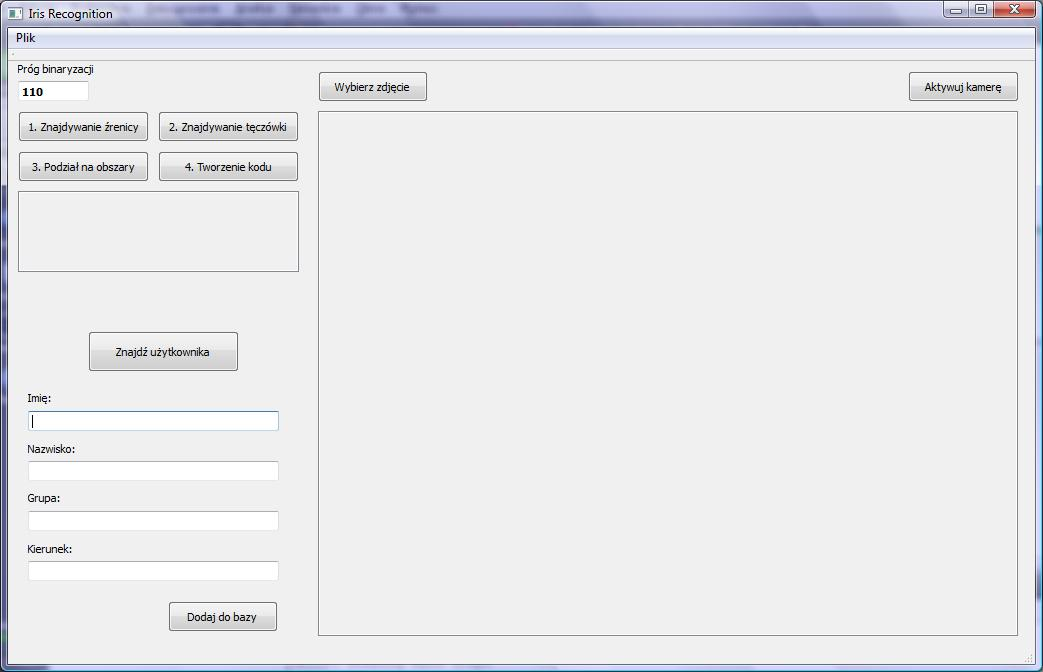
\includegraphics[scale=0.5]{okno_glowne.jpg}
\caption{Główne okno programu}
\label{fig:oknoGlowne}
\end{center}
\end{figure}

W przypadku uruchamiania systemu biometrycznej kontroli dostępu po raz pierwszy, możliwe jest jedynie dodawanie użytkowników do bazy w~sposób podstawowy, niezapewniający funkcji przyporządkowywania osób istniejącym kierunkom, przedmiotom i~grupom. Jest to spowodowane początkowym brakiem danych w~tabelach odpowiedzialnych za przechowywanie niesionych z~tym informacji. Wypełnienie pól znajdujących się w~głównym oknie aplikacji, przedstawionym na obrazku \ref{fig:oknoGlowne}, powoduje uzupełnienie wyłącznie wybranych atrybutów w~tabelach \verb!Students!, \verb!Biometrics!, \verb!Groups! i~\verb!Faculties!.

Interfejs użytkownika systemu został rozwinięty o~zbiór zakładek, pozwalających na wprowadzanie danych do bazy zgodnie ze schematem na rysunku \ref{fig:etapyDzialania}. Dostępne są one po naciśnięciu przycisku Zaawansowane opcje dodawania, widocznym na rysunku \ref{fig:oknoGlowne}.

Opis danych wprowadzanych do bazy podczas uzupełniania kolejnych zakładek został przedstawiony w akapitach dotyczących każdej zakładki.  


Pierwszą zakładką, umożliwiającą uzupełnienie bazy o~nowe informacje, jest \textbf{Dodaj kierunek}, pokazana na rysunku \ref{fig:dodajSpecjalizacje}. Składa się ona z~pól \verb!Nazwa kierunku! i~\verb!Nazwa wydziału!. W~celu dodania nowego kierunku do bazy, należy uprzednio wprowadzić nazwę wydziału, z~którym kierunek będzie powiązany, a następnie zatwierdzić zmiany. Po wybraniu wydziału z~listy, można wpisać nazwę kierunku. Aby zmodyfikować istniejący kierunek, należy wybrać z~listy rozwijalnej nazwę wydziału, a następnie nazwę zmienianego kierunku. Pola zakładki zostały wyposażone w~podpowiedzi, pełniące funkcje pomocy w~przypadku, gdy użytkownik nie jest pewny, jakiej postaci powinny być wpisywane dane. 

\begin{figure}
\begin{center}
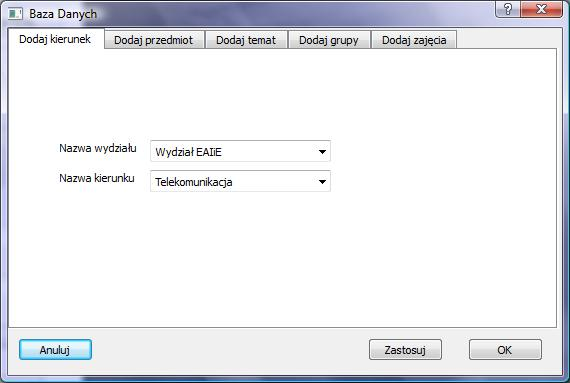
\includegraphics[scale=0.7]{dodaj_kierunek.jpg}
\caption{Zakładka do dodawania wydziałów i~kierunków}
\label{fig:dodajSpecjalizacje}
\end{center}
\end{figure}

W~trakcie dodawania kierunku bądź edycji już istniejącego, wraz z~wypełnieniem pól i~potwierdzeniem wpisywanych informacji, uzupełniane lub modyfikowane są następujące atrybuty w bazie danych:
\begin{itemize}
\item W tabeli Wydziały (\verb!Faculties!):
\begin{itemize}
\item Nazwa wydziału (\verb!faculty!) - pole z~nazwą wydziału,
\item Identyfikator wydziału (\verb!faculty_id!) - pole z~unikatowym identyfikatorem wydziału.
\end{itemize}
\item W tabeli Kierunki (\verb!Specialisations!):
\begin{itemize}
\item Kierunek (\verb!specialisation!) - jest to pełna nazwa kierunku; pole to jest jednym z~wymaganych przy wprowadzaniu informacji,
\item Wydział (\verb!faculty_id!) - identyfikator wydziału; pole jest wymagane,
\item Identyfikator kierunku (\verb!specialisation_id!) - jest to unikalne pole, identyfikujące kierunek wśród innych w~sposób jednoznaczny; nie wymaga ono bezpośredniego wprowadzania wartości przez użytkownika, gdyż jest automatycznie uzupełniane przy tworzeniu nowego rekordu, dlatego też w~interfejsie aplikacji nie ma specjalnego miejsca dla wprowadzenia danych odnoszących się do niego.
\end{itemize}
\end{itemize}

\begin{figure}
\begin{center}
\includegraphics[scale=0.7]{faculties.jpg}
\caption{Tabela Wydziały}
\label{fig:faculties}
\end{center}
\end{figure}
\begin{figure}
\begin{center}
\includegraphics[scale=0.7]{specialisations.jpg}
\caption{Tabela Kierunki}
\label{fig:specialisations}
\end{center}
\end{figure}


Następną zakładką dającą możliwość wprowadzania danych jest \textbf{Dodaj przedmiot}. Posiada ona pola \verb!Wydziału!, \verb!Kierunku!, \verb!Nazwy przedmiotu! oraz \verb!Roku studiów!, w~trakcie którego przedmiot jest prowadzony. Nazwy wydziału i~kierunku można wybrać z~list rozwijalnych. Po wybraniu wydziału, istnieje możliwość wyboru wyłącznie kierunków związanych z~danym wydziałem. W~celu zmiany danych istniejącego w~bazie przedmiotu, można wybrać go z~listy w~polu Nazwy przedmiotu, wówczas pole Rok studiów ulegnie uzupełnieniu informacjami. Podobnie jak w~przypadku dodawania kierunku, również w~tej zakładce dostępna jest pomoc dla użytkownika w~postaci pojawiających się podpowiedzi. 

\begin{figure}
\begin{center}
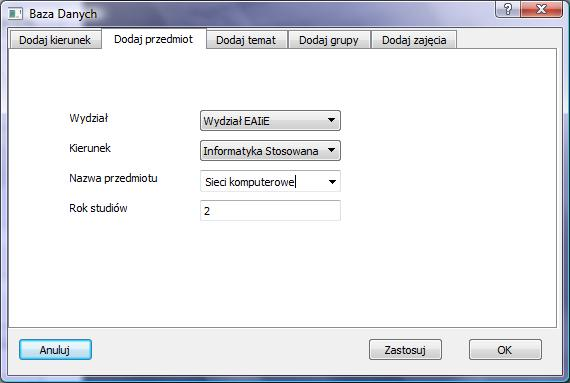
\includegraphics[scale=0.7]{dodaj_przedmiot.jpg}
\caption{Zakładka do dodawania przedmiotów}
\label{fig:dodajPrzedmiot}
\end{center}
\end{figure}

 Podczas wprowadzania przedmiotu lub edycji informacji dotyczących istniejącego, w~efekcie potwierdzenia danych wpisanych w~odpowiednich polach, uzupełnieniu ulegają następujące atrybuty tabeli Przedmioty (\verb!Subjects!):
\begin{itemize}
\item Przedmiot (\verb!subject!) - pełna nazwa przedmiotu; jest to pole wymagane,
\item Kierunek (\verb!specialisation_id!) - pole zawierające identyfikator kierunku, na którym prowadzony jest przedmiot; jest ono uzupełniane poprzez wybranie nazwy kierunku i~wydziału z~listy, które są przekształcane na odpowiedni identyfikator charakteryzujący kierunek w~tabeli Kierunki,
\item Rok studiów (\verb!year_of_studies!) - rok studiów kierunku, podczas którego prowadzony jest dany przedmiot
Identyfikator przedmiotu (\verb!subject_id!) - jest to unikalny identyfikator dla przedmiotu w~obrębie tabeli.
\end{itemize}

\begin{figure}
\begin{center}
\includegraphics[scale=0.7]{subjects.jpg}
\caption{Tabela Przedmioty}
\label{fig:subjects}
\end{center}
\end{figure}

W zakładce \textbf{Dodaj temat}, przedstawionej na rysunku \ref{fig:dodajTemat}, możliwe jest dodawanie tematów realizowanych w~obszarze danego przedmiotu. Dostępne pola na tej zakładce to \verb!Wydział!, \verb!Kierunek!, \verb!Przedmiot! oraz \verb!Nazwa tematu!. Pole nazwy tematu należy uzupełnić wybranymi danymi. W~przypadku edycji istniejącego tematu, można wybrać go z~listy takiej, jak w~polach nazw wydziału, kierunku i~przedmiotu.

\begin{figure}
\begin{center}
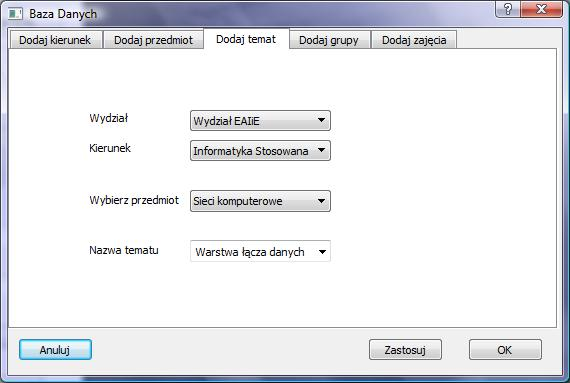
\includegraphics[scale=0.7]{dodaj_temat.jpg}
\caption{Zakładka do dodawania tematów}
\label{fig:dodajTemat}
\end{center}
\end{figure}

Po uprzednim wypełnieniu pól i~zatwierdzeniu wpisywanych informacji, uzupełniane są następujące atrybuty tabeli Tematy (\verb!Topics!) w~bazie danych:
\begin{itemize}
\item Temat (\verb!topic!) - pełna nazwa wprowadzanego tematu,
\item Przedmiot (\verb!subject_id!) - pole identyfikatora przedmiotu, w~obrębie którego dodawany jest temat; po wybraniu przez użytkownika nazwy przedmiotu, kierunku, wydziału i~roku, na których jest prowadzony, następuje wyszukanie odpowiadającego im identyfikatora w~tabeli Przedmioty,
\item Identyfikator tematu (\verb!topic_id!) - unikalny identyfikator tematu, automatycznie tworzony podczas wprowadzania danego tematu; nie wymaga on bezpośredniego wpisywania danych przez użytkownika, dlatego nie posiada odpowiadającego mu pola w~aplikacji.
\end{itemize}

\begin{figure}
\begin{center}
\includegraphics[scale=0.7]{topics.jpg}
\caption{Tabela Tematy}
\label{fig:topics}
\end{center}
\end{figure}

Kolejna zakładka o~nazwie \textbf{Dodaj grupę}, umożliwia tworzenie grup studentów uczęszczających na zajęcia z~przedmiotów. Pola niezbędne do wypełnienia na niej to \verb!Wydział!, \verb!Kierunek!, \verb!Przedmiot!, \verb!Dzień! odbywania się zajęć (do wybrania z~listy dni tygodnia), \verb!Godzina! odbywania się zajęć (w formie GG:MM, gdzie GG odpowiada godzinie, a MM minutom) oraz \verb!Nazwa grupy!. W~przypadku nazwy tej wymagane jest, aby była ona różna od wszystkich innych nazw grup obecnych w~bazie.

\begin{figure}
\begin{center}
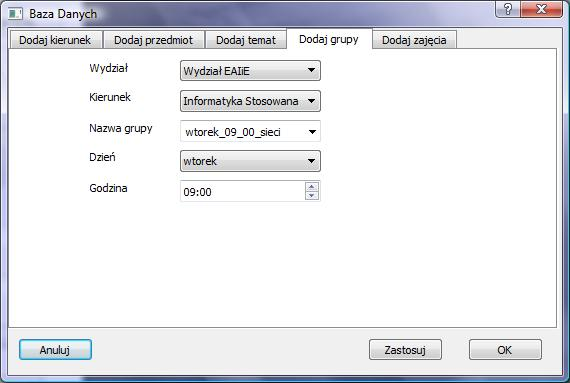
\includegraphics[scale=0.7]{dodaj_grupe.jpg}
\caption{Zakładka do dodawania grup}
\label{fig:dodajGrupe}
\end{center}
\end{figure}

 Wraz z~potwierdzeniem wpisywanych informacji, do bazy wprowadzeniu ulegają wartości następujących atrybutów tabeli Grupy (\verb!Groups!):
\begin{itemize}
\item Identyfikator przedmiotu (\verb!subject_id!) - pole zawierające informacje na temat przedmiotu, w~obrębie którego tworzona jest dana grupa; na podstawie wybranych informacji wyszukiwany jest identyfikator przypisany do przedmiotu w~tabeli Przedmioty,
\item Dzień odbywania się zajęć (\verb!day_of_week!) - dzień tygodnia, w~którym odbywać się będą zajęcia grupy,
\item Godzina odbywania się zajęć (\verb!time_of_classes!) - godzina odbywania się zajęć danej grupy,
\item Nazwa grupy (\verb!group_name!) - nazwa grupy,
\item Identyfikator grupy (\verb!group_id!) - identyfikator jednoznacznie określający grupę w~tabeli; jest to wartość tworzona automatycznie, nie wymaga wprowadzania informacji od użytkownika.
\end{itemize}

\begin{figure}
\begin{center}
\includegraphics[scale=0.7]{groups.jpg}
\caption{Tabela Grupy}
\label{fig:groups}
\end{center}
\end{figure}

Następna zakładka pozwalająca na uzupełnienie bazy danych to \textbf{Dodaj zajęcia}. Obecne na niej pola \verb!Wydziału!, \verb!Kierunku!, \verb!Przedmiotu! oraz \verb!Grupy! umożliwiają wprowadzenie do bazy zajęć odbywających się w~terminie wybranym w~polu \verb!Data zajęć!, podczas których realizowany będzie określony temat. W~zakładce tej również pojawiają się podpowiedzi informujące o~formie wprowadzanych nazw i~daty.

\begin{figure}
\begin{center}
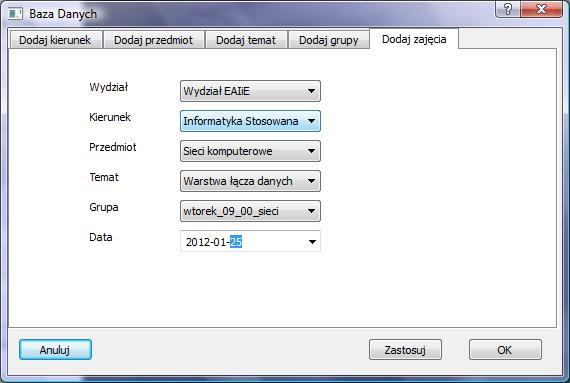
\includegraphics[scale=0.7]{dodaj_zajecia.jpg}
\caption{Zakładka do dodawania zajęć}
\label{fig:dodajZajecia}
\end{center}
\end{figure}

 Wprowadzenie danych w polach zakładki powoduje uzupełnienie tabeli Zajęcia (\verb!Classes!), która posiada atrybuty:
\begin{itemize}
\item Przedmiot (\verb!subject_id!) - identyfikator przedmiotu, z~którego odbywać się będą zajęcia; jest on pobierany z~tabeli Przedmioty na podstawie wybranego pola,
\item Temat (\verb!topic_id!) - identyfikator tematu, który będzie realizowany na danych zajęciach,
\item Grupa (\verb!group_id!) - identyfikator grupy, do której przypisane będą zajęcia,
\item Data (\verb!class_date!) - termin zajęć,
\item Kierunek (\verb!specialisation_id!) - identyfikator kierunku, w~skład którego wchodzą użytkownicy z~danej grupy,
\item Identyfikator zajęć (\verb!class_id!) - unikalny identyfikator zajęć.
\end{itemize}

\begin{figure}
\begin{center}
\includegraphics[scale=0.7]{classes.jpg}
\caption{Tabela Zajęcia}
\label{fig:classes}
\end{center}
\end{figure}

Po uzupełnieniu bazy kierunkami, przedmiotami, grupami, tematami i~zajęciami można przystąpić do dodawania użytkowników. W~tym celu potrzeba wypełnić w~oknie głównym programu pola \verb!Imię!, \verb!Nazwisko!, \verb!Kierunek! i~\verb!Grupa!, w~formie ręcznego wprowadzania danych bądź wyboru informacji z~listy.

Po uzupełnieniu pól, odpowiednim atrybutom tabel Studenci (\verb!Students!) oraz Grupy studentów (\verb!Students_Groups!) nadawane są wartości:
\begin{itemize}
\item W tabeli Studenci:
\begin{itemize}
\item Imię (\verb!name!) - pełne imię użytkownika,
\item Nazwisko (\verb!surname!) - pełne nazwisko studenta,
\item Kierunek (\verb!specialisation_id!) - informacje dotyczące kierunku studiów; po wybraniu opcji z~listy kierunków umieszczonych w~bazie Kierunki, przyporządkowany zostaje identyfikator kierunku, opisujący go w~sposób unikalny,
\item Przedmiot (\verb!subject_id!) - dane przedmiotu, do którego zostanie przypisany student; wybrane informacje ulegają przekształceniu na identyfikator przedmiotu w~tabeli Przedmioty,
\item Grupa (\verb!group_id!) - nazwa grupy z~przedmiotu, do której będzie przypisany student; na podstawie nazwy tej uzupełniany jest identyfikator danej grupy,
\item Identyfikator studenta (\verb!student_id!) - unikalny identyfikator dla osoby w~obrębie całej tabeli,
\item Identyfikator biometryki (\verb!biometrics_id!) - identyfikator biometryki, tworzonej dla każdego studenta.
\end{itemize}
\item W tabeli Grupy studentów:
\begin{itemize}
\item Identyfikator grupy (\verb!group_id!) - identyfikator grupy przedmiotu,
\item Identyfikator studenta (\verb!student_id!) - identyfikator studenta, który jest tworzony i~automatycznie przypisywany do grupy o~wymienionym identyfikatorze \verb!group_id!.
\end{itemize}
\end{itemize}

\begin{figure}
\begin{center}
\includegraphics[scale=0.7]{students.jpg}
\caption{Tabela Studenci}
\label{fig:studens}
\end{center}
\end{figure}
\begin{figure}
\begin{center}
\includegraphics[scale=0.7]{studentsgroups.jpg}
\caption{Tabela Grupy studentów}
\label{fig:studentsgroups}
\end{center}
\end{figure}

Podstawową funkcją tabeli Grupy studentów jest połączenie informacji przechowywanych w~tabelach Studenci oraz Grupy. Podczas dodawania kolejnych osób do grupy o~danej nazwie, następuje uzupełnianie tabeli Grupy studentów rekordami o~tym samym identyfikatorze grupy, ale różnych identyfikatorach studentów, co powoduje przypisanie wielu osób do tej samej grupy.

Aby przypisać użytkownikowi biometrykę, należy postępować zgodnie z~instrukcją przedstawioną w~dalszych częściach pracy.

Pierwszym wymaganym krokiem jest opisane uzupełnienie danych użytkownika. Niezbędne jest również pobranie zdjęcia dodawanego użytkownika lub wczytanie  go z~nośnika danych. Następnie należy wcisnąć przycisk Dodaj do bazy. Spowoduje to otwarcie okienka z~wynikiem segmentacji obszaru tęczówki, który powinien być zweryfikowany przez użytkownika. Po pozytywnej weryfikacji utworzony zostaje kod tęczówki danej osoby.

 Tabelą gromadzącą kody tęczówek jest tabela Biometryki (\verb!Biometrics!). Składa się ona z~następujących atrybutów:
\begin{itemize}
\item Kod tęczówki (\verb!iris_pattern!) - pole przechowujące informacje o~utworzonym kodzie tęczówki ,
\item Odcisk palca (\verb!fingerprint_pattern!) - dodatkowe pole przechowujące kod odcisku palca, które mogłoby być wykorzystane w~przypadku rozbudowy systemu o~funkcjonalność rozpoznawania na tej podstawie,
\item Kod twarzy (\verb!face_pattern!) - pole przechowujące informacje dotyczące kształtu twarzy, używane w~przypadku poszerzenia systemu o~identyfikację w~oparciu o~kształt twarzy,
\item Identyfikator biometryki (\verb!biometrics_id!) - identyfikator charakteryzujący biometrykę.
\end{itemize}

\begin{figure}
\begin{center}
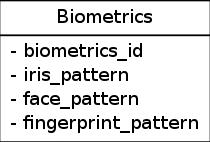
\includegraphics[scale=0.7]{biometrics.jpg}
\caption{Tabela Biometryki}
\label{fig:biometrics}
\end{center}
\end{figure}

Tabelą pomocniczą dla tabeli Biometryki jest Zdjęcia (Photos). Posiada ona atrybuty:
\begin{itemize}
\item \verb!iris_1 .. iris_5! - pole przechowujące pobrane zdjęcia tęczówki oka, służące do tworzenia kodu tęczówki,
\item \verb!finger_1 .. finger_5! - pola służące do przechowywania zdjęć odcisków palca, w~przypadku, gdy system zostanie poszerzony o~funkcjonalność identyfikacji na podstawie odcisków palców,
\item \verb!face_1 .. face_5! - pola przechowujące fotografie twarzy, w~przypadku, gdy system posiada funkcjonalność rozpoznawania na podstawie kształtu twarzy.
\end{itemize}

\begin{figure}
\begin{center}
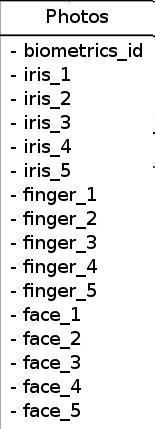
\includegraphics[scale=0.7]{photos.jpg}
\caption{Tabela Zdjęcia}
\label{fig:photos}
\end{center}
\end{figure}

W celu sprawdzenia obecności użytkowników, wymagane jest pobranie zdjęć poszczególnych osób i~wyznaczenie kodów tęczówek potrzebnych do ich identyfikacji. W~przypadku pozytywnej identyfikacji danej osoby pola danych osobowych ulegają uzupełnieniu. Można wówczas wybrać zajęcia, na których obecna jest osoba, oraz ewentualnie temat odrabianych zajęć, jeśli jest to student odrabiający. W~przypadku nierozpoznania osoby, wyświetlany jest odpowiedni komunikat informujący o nieznalezieniu danych identyfikowanego użytkownika.

Tabelami umożliwiającymi uzupełnienie list obecności oraz osób odrabiających zaległe tematy są Obecność (Attendance) i~Odrabiający (Complements). Posiadają one pola:
\begin{itemize}
\item Tabela Obecność:
\begin{itemize}
\item Identyfikator zajęć (\verb!class_id!) - identyfikator zajęć, na których obecny lub nieobecny jest użytkownik,
\item Identyfikator studenta (\verb!student_id!) - identyfikator użytkownika.
\end{itemize}
\item Tabela Odrabiający:
\begin{itemize}
\item Identyfikator zajęć (\verb!class_id!) - identyfikator zajęć, które osoba odrabia,
\item Identyfikator studenta (\verb!student_id!) - identyfikator użytkownika,
\item Data uzupełniania zajęć (\verb!complement_date!) - data odrabiania danych zajęć.
\end{itemize}
\end{itemize}

\begin{figure}
\begin{center}
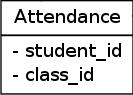
\includegraphics[scale=0.7]{attendance.jpg}
\caption{Tabela Obecność}
\label{fig:attendance}
\end{center}
\end{figure}
\begin{figure}
\begin{center}
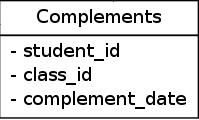
\includegraphics[scale=0.7]{complements.jpg}
\caption{Tabela Odrabiający}
\label{fig:complements}
\end{center}
\end{figure}


Program umożliwia również generację list obecności na danych zajęciach. Funkcja ta jest dostępna przy użyciu przycisku Generuj listę obecności.

\section{Zastosowane technologie}
\label{sec:implementacja}

Podczas rozbudowy podstawowej wersji aplikacji użyto technologii zaproponowanych w~pracy \cite{Gl11}, ze względu na oferowane przez nie zalety. Jedynie w~procesie projektowania bazy danych zdecydowano się na wdrożenie odmiennej technologii. Spowodowane to było niedostępnością sterownika do obsługi systemu zarządzania bazą danych MySQL w~używanym środowisku programistycznym, stosowanym do zaprojektowania systemu.

Językiem programowania, użytym podczas implementacji obsługi bazy danych, był C++. Jest to rozbudowany, obiektowy język oferujący wiele różnych bibliotek. Użytą biblioteką do obsługi bazy danych oraz tworzenia interfejsu jest Qt. C++ posiada bogate API, co ułatwia korzystanie z~gotowych funkcji interfejsu.

Środowiskiem programistycznym służącym do tworzenia aplikacji był QtCreator, z~wbudowaną biblioteką Qt w~wersji 4. Biblioteka ta umożliwia tworzenie zaawansowanych interfejsów użytkownika przy użyciu gotowych kontrolek i~form, bez konieczności budowania GUI od podstaw.

Wśród wielu technologii bazodanowych, najlepszą okazała się być SQLite. Nie wymaga ona uruchamiania serwera bazy danych i~wszystkie dane przechowywane są w~jednym pliku. W~związku z~tym, aplikację można uruchomić w~każdym miejscu. Zdefiniowane w~niej rodzaje struktur przechowywanych danych są wystarczające do realizowanych celów.
